\label{sec:implementation}

This section presents our design of the cell view. We first introduce different components of a cell view and their implementations in Sec.~\ref{sec:components}. Then we present in Sec.~\ref{sec:mapping} the detailed mapping schemes that encode the various attributes to properties of simple geometric shapes. In Sec.~\ref{sec:timeline} we present a layout algorithm inspired from fast tone-mapping technique to avoid cluttered drawing on the timeline.  

\subsection{Components}
\label{sec:components}
A cell view has three basic components: a timeline, a disk panel and a set of cilia.  

\textbf{Timeline.} The time line is an directional open curve joined by an circular arc and a quadratic Bezier curve. The arc is of radius $R$, centered on screen and spanning an angle from $\delta$ to $2\pi-\delta$, where $\delta$ is set to a small positive value ($\frac{\pi}{12}$ in our work) to differentiate the starting point from the end point. The control points of the Bezier curve are specified by $\delta$ and $R$ in order to let the curve joins the arc with tangent continuity.

%\begin{figure}[h!]
%	\centering
%		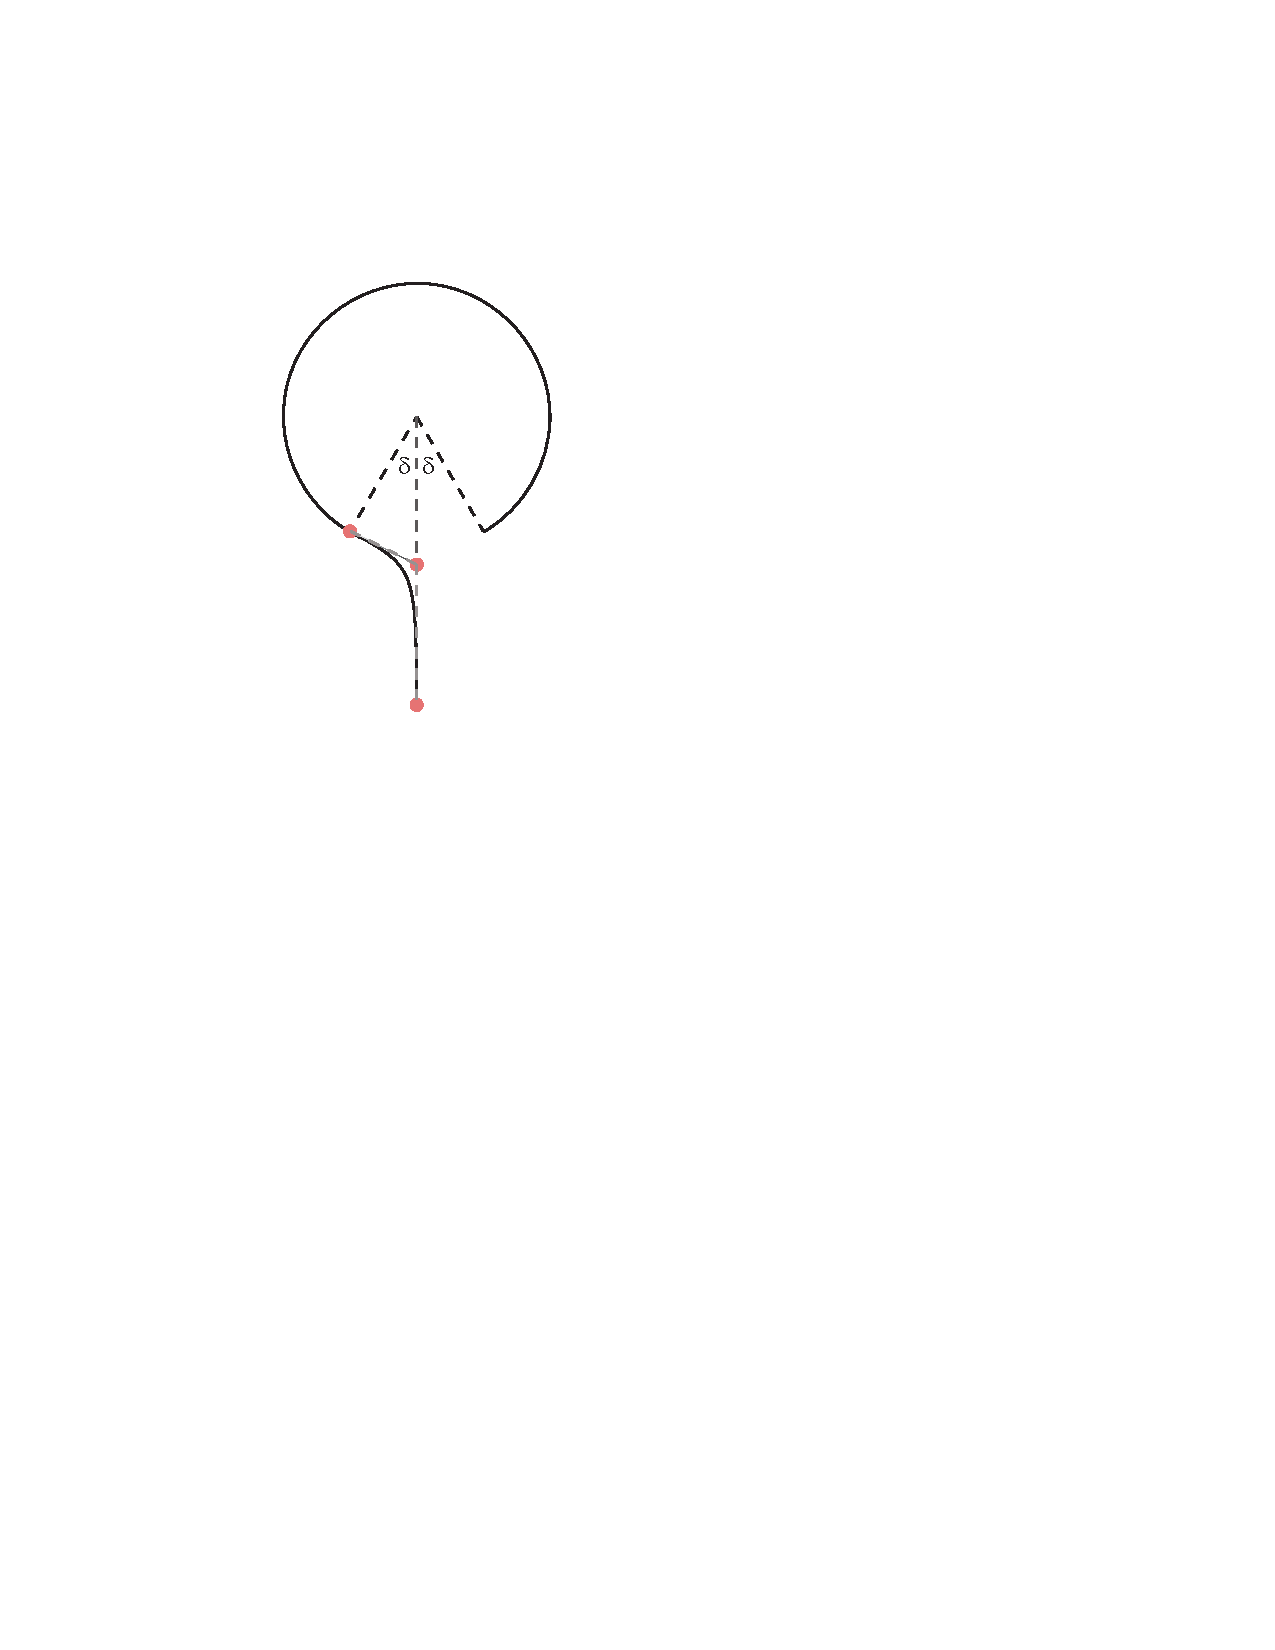
\includegraphics[width=1.3in]{pics/timeline.pdf}
%	\label{fig:timeline}
%	\caption{The timeline is an open curve joined by an arc and a quadratic Bezier curve: the red dots are the control points of the Bezier curve.}
%\end{figure}

The use of circular timeline is not new~(e.g.~\cite{Chuah:1998}) and is commonly appeared as a model in geology and news data visualization for presenting events that are evolving or periodic in nature. Here the motivation is to view malware network traces as an entity. We believe that using a circular timeline instead of a straight timeline better promotes this impression.

\textbf{Disk Panel.} The circular timeline delimits a round area which is used to display the primary key of the malware instance or details of a user-selected stream. In the viewing mode, the unique MD5 value is shown on the disk panel. In the interaction mode, the disk panel display attribute values of the user-selected stream. It is possible to show the details of a stream near the cilium representing this stream, or in another pop-up panel; nevertheless, using the disk panel is a more economical choice in terms of minimizing the total screen space necessary for the view. 

\textbf{Cilium.} Each cilium represents a stream of network communications. A cilium has a \emph{stem} and a \emph{head}. The stem of the cilium is a quad strip. Each quad represent a packet and hence the longer the stem the larger is the number of packets being transmitted. The width of the stem is correlated with the duration of the stream. The head of the cilium is a ellipse whose width encodes the size of transmission. Note that in a real-world scenario, the number of packets, duration and size are highly correlated with each other. Hence, the width of a cilium's head commonly scales with the length of its stem. Outliers, such as a 'short' cilium with a 'wide' head or a 'tall' cilium with a 'slender' stem , might be indicative of interesting behavior.     

\textbf{Drawing.} All geometric dimensions~(timeline radius, cilium height, width, etc.) are relative to the screen size, hence the cell view can scale without loss of quality. Each cilium object is associated with a drawing function~(\verb+drawCilium()+) that display the cilium with transparency in the local coordinate system. The transformation matrix stack is used to draw a cilium in the global coordinate system.
%\begin{verbatim} 
%pushMatrix(); 
%translate(P.x, P.y); 
%rotate(a); 
%drawCilium(); 
%popMatrix();
%\end{verbatim}
%where $P$ is the contact point of the cilium on the timeline determined the plan angle $a$ and the timeline's center $O$ and radius $R$.  

\subsection{Attribute Mapping}
\label{sec:mapping}
As expressed earlier, we use nonlinear mapping functions to transfer attribute values to geometric properties since linear mapping may require unbounded area. The design guideline of each mapping function is to limit each geometric dimension to be within a lower bound and a upper bound and is a monotonically increasing function of the input attribute value.   

\textbf{Mapping number of packets~$n$ to cilium stem height~$h$:} The stem of the cilium is a quad strip where each quad denotes a packet. The cilium height $h$ is the sum of the set of quad heights $\{h_i\}$, which forms a geometric sequence with $r$ as the scale factor:
\[ r = \frac{h_{max} - h_{min}}{ h_{max}} \]
For example, if a stream has $n$ packets, the height of its stem is
\begin{equation}
h = h(n) = \sum_{i=1}^n h_i = h_{max}(1-r^n)
\end{equation}
Hence, $h$ is bounded by $h_{min}$ and $h_{max}$, and $h(n)$ is monotonically increasing in $n$. 

\textbf{Mapping duration~$t$ to cilium stem width~$w$:} The width $w$ of the stem is mapped from the duration $t$ of the stream by the following transfer function
\begin{equation}
w = w(t) = w_{max} -  \frac{w_{max} - w_{min}}{t+1}
\end{equation}
This would limit the width of the stem to $w_{max}$ and $w(t)$ is a increasing function of $t$. 

\textbf{Mapping size of transmission~$z$ to cilium head width~$w$:} Similarly, the width $l$ of the oval head of the stem is computed from the size of the stream, denoted by $z$:
\begin{equation}
l = l(z) = l_{max} - \frac{l_{max} - l_{min}}{log(z)}
\end{equation}
As the sizes of transmission of different streams can be drastically different~(ranges from $10^2$ to $10^6$ bytes), we use logarithm of $z$ in the mapping function. 

\subsection{Layout on Timeline}
\label{sec:timeline}
To strengthen the visualization as a cell entity, we clock-wisely oriented the set of streams around the circular timeline. Each stream has a starting time which we denote as $s_i$, and the position it appears on the circular timeline is determined by its contacting angle $a_i$. The relative order and the intermissions of a set of streams are important characteristics of a malware instance's behavior.  
     
Therefore, given a set of starting times $\{s_i\}, i=1,...,k$, we want to compute a set of angles $\{a_i\}$ bounded by the mappable range $[ \delta, 2\pi-\delta]$. Assume that $\{s_i\}$ is sorted. $s_1$ is the smallest and mapped to $\delta$ and $s_k$ is the largest and mapped to $2\pi-\delta$. As mentioned earlier, the distribution of $\{s_i\}$ is very uneven because multiple streams of communications may occur in a very short time period. Hence, linearly mapping $\{s_i\}$ to the mappable range may lead to overlappings and visual clutter, as shown in Fig.~\ref{fig:Tune}~left. In order to improve clarity while preserving the relative order as they appear in $\{s_i\}$, we present a recursive range mapping algorithm in Alg.~\ref{alg:mapping}. This algorithm is inspired by fast tone reproduction techniques for visualizing high dynamic range image data~\cite{Duan:2004} based on the fact that the distribution of HDR data tends to be sparse. Here, the set of starting times $\{s_i\}$ is analogous to the raw HDR image data and the mappable range~($[ \delta, 2\pi-\delta]$) is analogous to the viewable intensity range~($[0, 255]$) in the tone-mapped image. The idea of fast tone-mapping is to scale the mapping range according to the input data histogram: the time period that contains more incidences of streams is mapped to a larger range. 
  
\textbf{Algorithm Tuning.} Specifically, $\alpha \in [0, 1]$ is the parameter that specifies the scaling effect: the larger $\alpha$ is, the more equalized the mapping is. If $\alpha=0$, Alg.~\ref{alg:mapping} is essentially a linear mapping, which causes visual clutter due to that multiple streams typically start together. If $\alpha = 1$, Alg.~\ref{alg:mapping} is the equalized mapping where the streams appear uniformly spaced. However, the equalized mapping does not show intermissions, such as a long period of inactivity after the first DNS stream in Fig.~\ref{fig:Tune}~right.       

\begin{algorithm}
\floatname{algorithm}{Alg.}
\renewcommand{\algorithmicrequire}{\textbf{Input:}}
\renewcommand{\algorithmicensure}{\textbf{Result:}}
\caption{Recursive range mapping: $map(i, j, a_{min}, a_{max})$ }
\label{alg:mapping}
\begin{algorithmic}
\REQUIRE subarray indices $i,j$ of input array $s$, \\
         mapping range $[a_{min}, a_{max}]$ 
\ENSURE set angles in output array $a$
\STATE $a_{mean} \Leftarrow \frac{a_{min} + a_{max}}{2}$
\IF{$i \geq j$}
    \STATE $a_i \Leftarrow a_{mean}$
    \STATE return
\ENDIF
\STATE $s_{mean} \Leftarrow \frac{s_i+s_j}{2}$, 
\STATE $s_{median} \Leftarrow s_{(i+j)/2}$  
\STATE $cut \Leftarrow \alpha s_{median} + (1-\alpha)s_{mean}$
\STATE $ci\Leftarrow$ index of $cut$ in array $s$
\IF{$ci==i$}
	\STATE $a_i \Leftarrow a_{min}$
	\STATE $map(ci+1, j, a_{mean}, a_{max})$
	\STATE return
\ENDIF
\IF{$ci==j$}
	\STATE $a_j \Leftarrow a_{max}$
	\STATE $map(i, ci-1, a_{min}, a_{mean})$
	\STATE return
\ENDIF
\STATE $map(i, ci-1, a_{min}, a_{mean})$
\STATE $map(ci, j, a_{mean}, a_{max})$
\end{algorithmic}
\end{algorithm}


\begin{figure*}
	\centering
		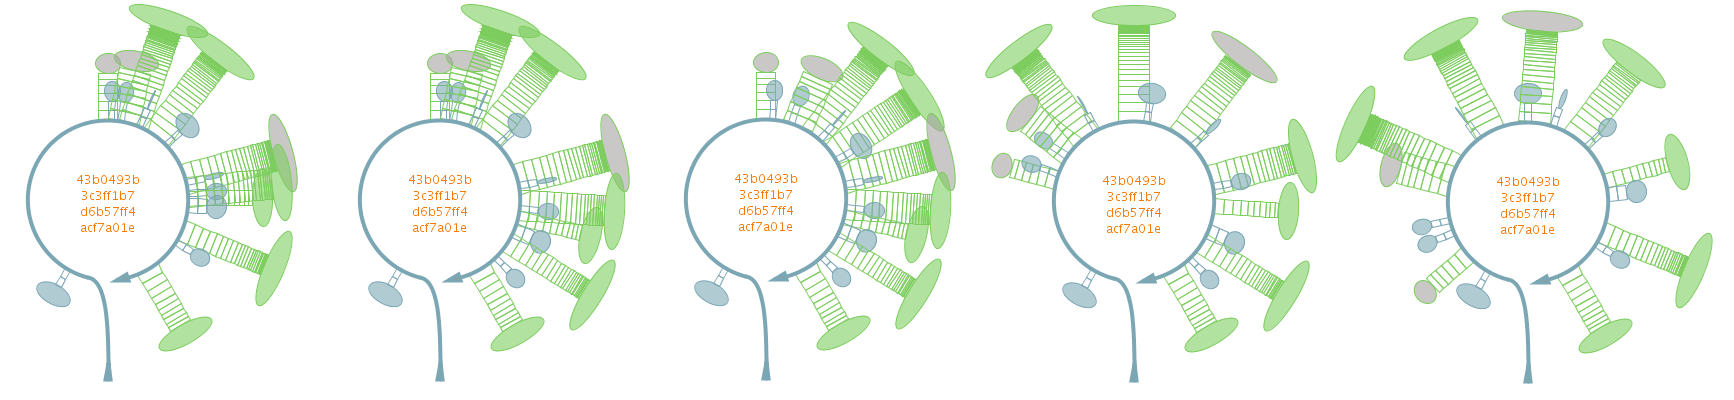
\includegraphics[width = 0.98\linewidth]{pics/Tune.png}
	\label{fig:Tune}
	\caption{From left to right, we show a sequence of visualizations of the same malware instance with increasing $\alpha$ values: (a) linearly mapping the starting times to angles would results in visual clutter; (d) equalized mapping helps to reduce the overlapping effects.}
\end{figure*}



